\chapter{Communication between mechanical and \acl*{fe} modelling}
\label{ch:modelling}
Mechanical and \acf{fe} modelling are closely linked.
Much of the work done in \ac{fe} modelling is a continuation or examination of phenomena observed in experimental modelling, and many experiments are conducted in support of \ac{fe} model validation.
A considerable portion of the work in this thesis was done in conjunction with the \ac{fe} modelling team under the supervision of Dr.\ Ben Helgason at ETH, Z\"{u}rich, Switzerland.
There was significant effort expended to ensure that the \ac{fe} modelling group had all the data required to create models that could be readily compared to the experiments performed.
This chapter gives a brief description of the data flow between the two modelling methods and efforts made on the experimental side to facilitate that flow.
Informally, we have dubbed this the \textit{data pipeline}.
I hope that future \ac{fe}-experiment collaborations can take advantage of my experience in this regard.

\section{Documentation from start to finish}
\label{sec:modelling_document}
The most critical aspect in creating an experiment that can be used for \ac{fe} validation is documentation and transparency.
From apparatus, to data and analysis routines, all aspects of the experiment must be fully described and accessible to the modelling community (Figure~\ref{fig:modelling_Dataflow}).

Details of experimental apparatus are useful in defining \acfp{bc} of \ac{fe} models.
The level of detail required in an \ac{fe} model may begin modestly, but as the model is refined researchers may need to integrate very high levels of detail in some aspects of the setup.
Since it cannot be easily anticipated where certain phenomena originate, experimental modellers must make an almost arbitrary level of detail available to the \ac{fe} modellers.
The purpose of an \ac{fe} model is frequently to examine aspect of the experiment that are difficult to explain based on current knowledge, which means that current knowledge should be used cautiously in determining what to include in a model.
As computational power increases, \ac{fe} researchers are including more apparatus in their models in an effort to close the gap between computational and experimental models; details provided by the engineers who designed the experimental apparatus can help the two models converge.

Computer code and analysis routines is another area where concerted effort to organize and communicate can pay off.
\ac{fe} researchers want data packed in a manner that makes data manipulation and extraction easy to automate.
Additionally, code annotation and inclusion of details like units used in a given portion of the analysis can be invaluable to an \ac{fe} modeller who is working remotely from the experimental researchers.
This kind of annotation and documentation of code is time consuming and can be challenging.
Experimentalists often use one-off custom code, with the routines designed to evaluate specific variables of concern for a given test.
Each researcher typically develops their own code, based on their own needs, that they understand well and rarely pass on to future experimentalists.
Computational researchers are used to developing and documenting code with the intent of passing it to the next researcher.
Indeed, very little progress would be made in the field if each \ac{fe} researcher had to start from scratch.
Additionally, in the computational world there is an understanding that no code is perfect, as evidenced by the continual releases of new versions of old software.
Experimentalists can be overtly aware of limitations, coding discrepancies and the nuances of running their software, which can make them reluctant to open-source it for fear of criticism~\citep{barnes_publish_2010}.
To address the latter fear, documentation must be an integral part of the analysis code development process, with the expectation that it will be released, along with the data, to another research group.
This was handled in the current work by developing a series of analysis classes that were portable and self contained (\S\ref{sec:code_dt_ins_analysis}).
Each class object contained the raw data, the final data, filtering and interpolation routines that yielded the final data, and routines to analyse and extract meaningful data, as well as variables concerned with those analyses.
This transparency and documentation allowed sending the data to researchers who were unfamiliar with the tests, and allowing them to access the full analysis, as well as documentation (including information like units) for each test and specimen.

\begin{figure}
\centering
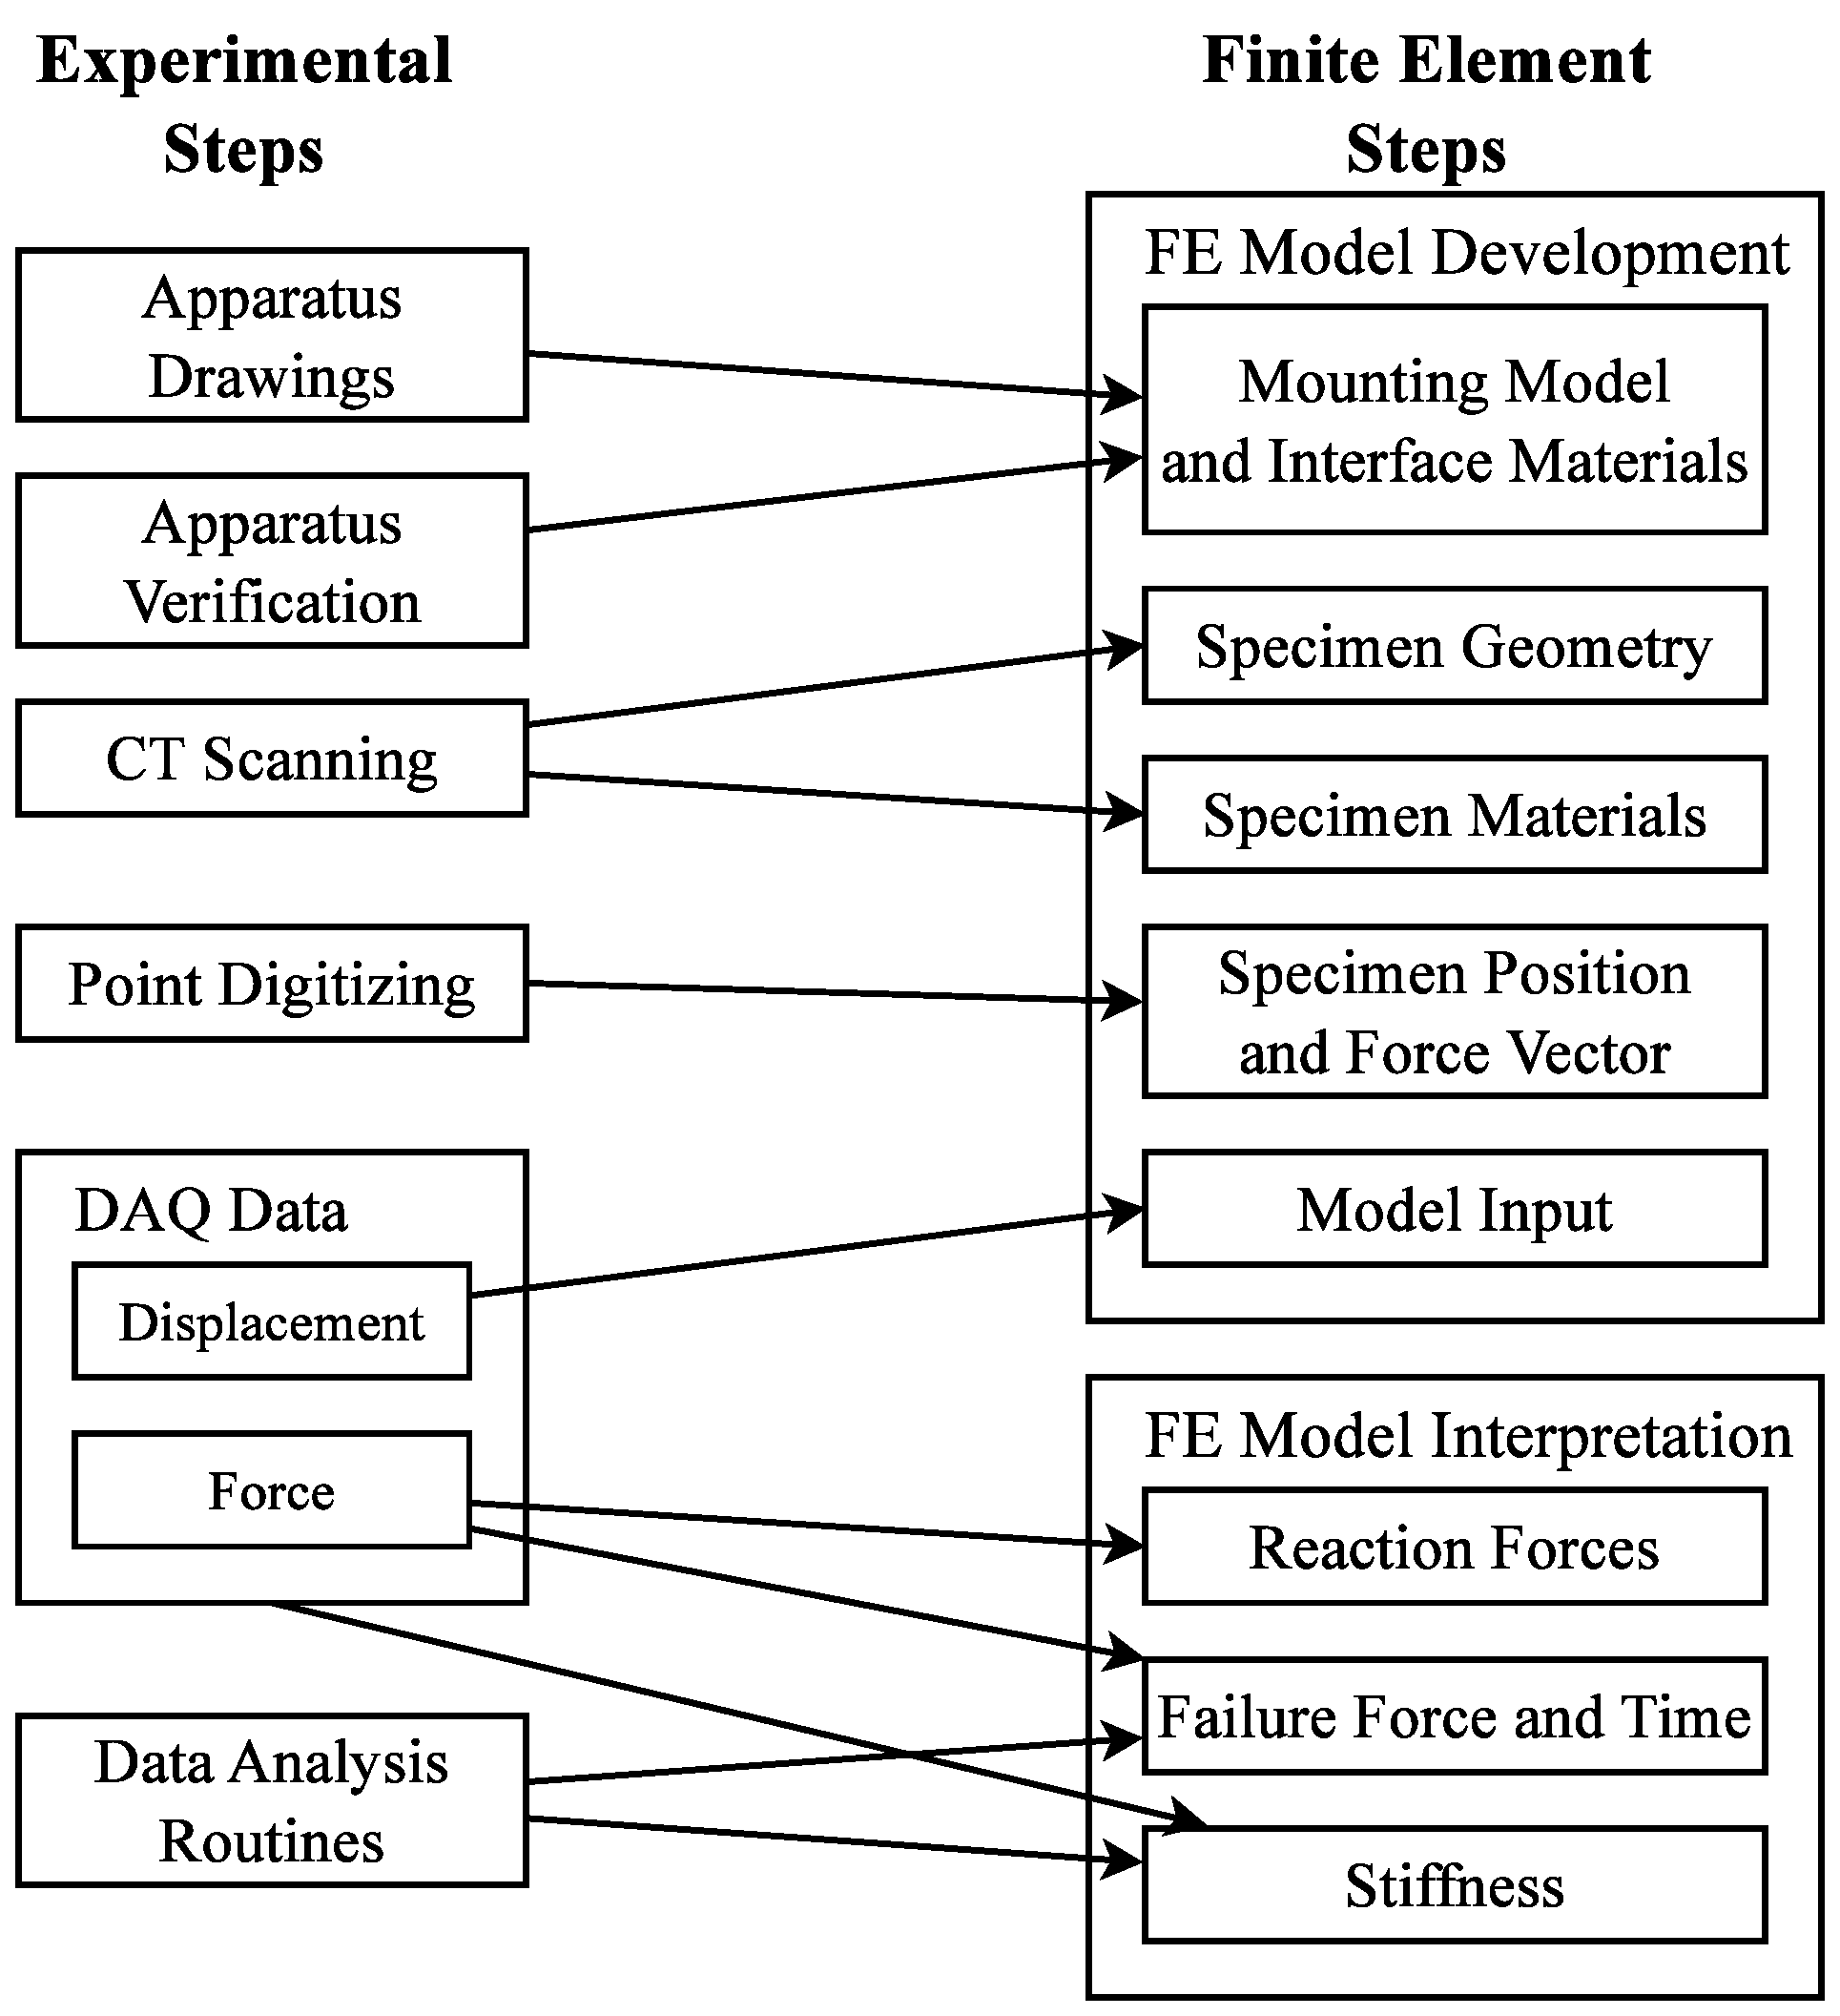
\includegraphics[height=\textwidth]{./testing_fe_modelling/figures/Dataflow}
\caption[Experimental and \acs*{fe} data flow]{\textbf{Flow of data between experimental and \ac{fe} modelling techniques. Documentation from the beginning is key and access to analysis routines is important for comparing data on an even footing.} Graphic \copyright Seth Gilchrist, 2013.}
\label{fig:modelling_Dataflow}
\end{figure}

\section{Additional data for \acs*{fe} modelling}
\label{sec:modelling_additional}
As mentioned in the previous section, the origins of phenomena observed in an experiment are often difficult to predict.
One potential source of obfuscation is poorly or incorrectly applied \acp{bc}.
This can be addressed by careful recording of experimental setup using technologies like \ac{ct}, surface digitization and landmark point digitization.
The majority of experimental models do not need for \ac{ct} imaging and surface topology of specimens.
\acs{a-p} radiographs and \ac{dxa} images are used by researchers to give a clinical context to the specimens being tested.
When working with \ac{fe} models, detailed geometric, densitometric and orientation data are needed, requiring collection of \ac{ct} images, as well as bone and test equipment landmarks.

Once the drawings of the apparatus, and geometry and density of the bones are obtained, an \ac{fe} model can be constructed and appropriate fixed boundary conditions applied.
The effector of an \ac{fe} model is typically a displacement or force \acl{bc}, the alignment of which is critical to the output of the model.
To align the force or displacement application in the computational model, the orientation of the bone during the actual experiment must be obtained.
This was done by collecting the (\textit{x,y,z}) coordinates of points on the surface of the bone and loading apparatus using an Optotrak (Certus, NDI, Ontario, Canada) with a digitization wand (Figure~\ref{fig:digitizing}).
Points were collected on each part of the specimen and apparatus and saved in a text file.
Approximately 30 points were taken on the femoral head, 30 on the femoral neck, 30 on the trochanter, 20 on the shaft, 20 on interface between each \ac{pmma} cup and the bone, 4 on the bottom platen, 6 on each side of the pivot, 8 on the impact hammer and finally 2 on the strain gauge.
The organization of the points was recorded in a log sheet (given in full in~\S\ref{sec:support_logsheets}) which was provided to the \ac{fe} modellers for reference.

\begin{figure}
\centering
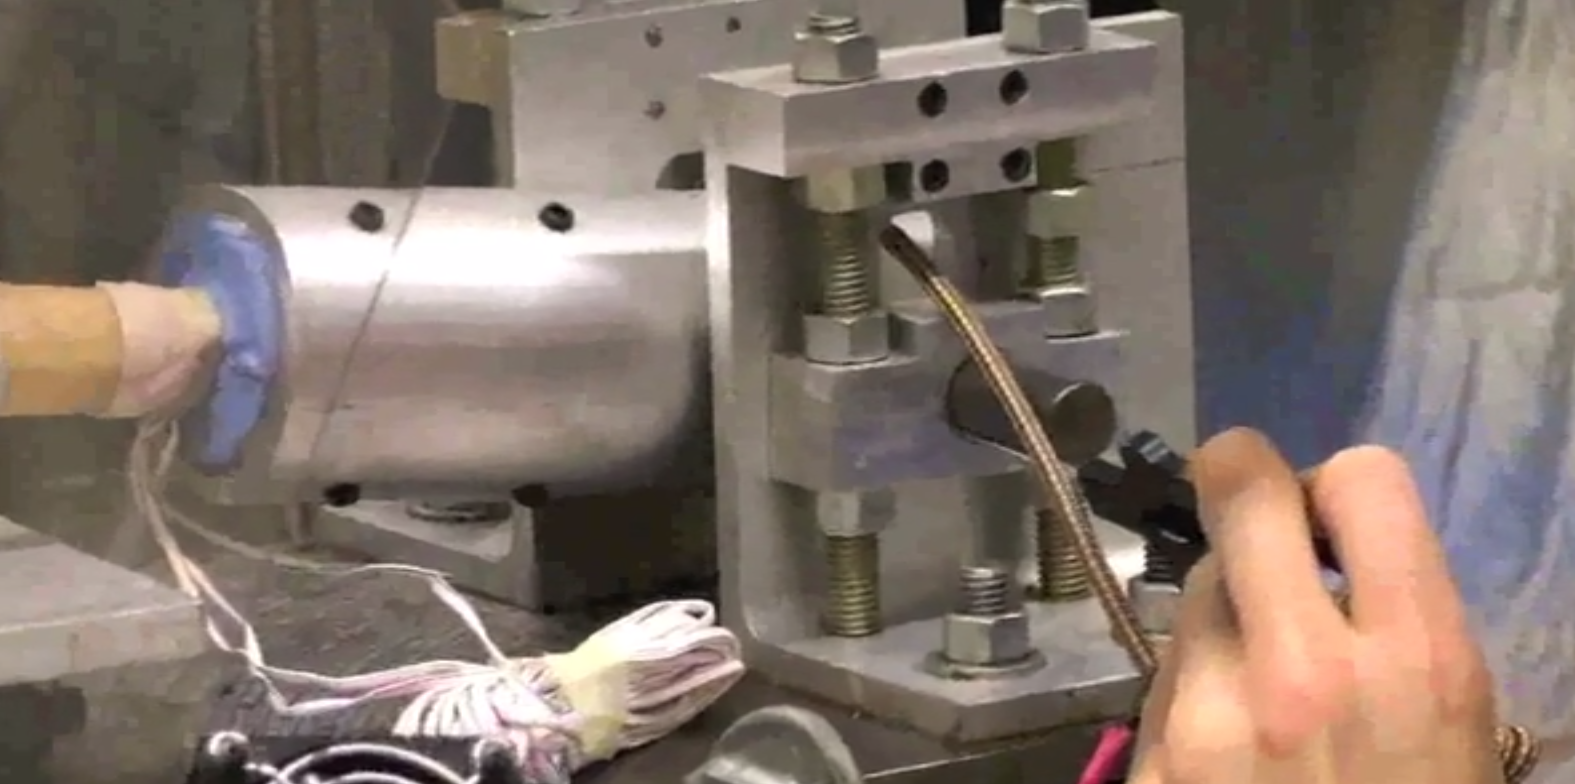
\includegraphics[width=\linewidth]{./testing_fe_modelling/figures/digitizing}
\caption[Digitizing points on the experimental apparatus]{\textbf{In this image, taken from a video of the setup procedure, the Optotrak digitizing wand is being used to digitize the location of the pivot at the distal end of the femoral shaft.} Image \copyright Seth Gilchrist, 2013.}
\label{fig:digitizing}
\end{figure}

\section{Data portability and transparency}
\label{sec:modelling_portable}
Data from the experiment are used to drive the \ac{fe} model and validate the output.
The models of the current tests, created by Oscar Ariza in Dr. Ben Helgason's facilities, used a velocity derived from the displacement data as the affecting \ac{bc}.
Other models may use a force \ac{bc}, but in any case, the modellers need to have access to the data and any filtering or post processing that was conducted.

The sources of the data, while important to a mechanical modeller, are of less importance to the computational community.
Instead, computational modellers are more concerned with consistency in data preparation and organization, allowing them to automate the process of extracting needed \acp{bc}.
For example, in the tests conducted in this thesis, displacement in the materials testing machine was recorded by a \ac{daq} from a voltage signal emitted by the materials testing machine, but in the fall simulator displacement was extracted from optical measurements of the trochanter and impact hammer.
Computational modellers would like the data to be accessed in a similar way, regardless of the fact that is was collected using different techniques.

Post processing of the data is important to both computational and mechanical modellers.
\ac{fe} modellers obtain force and displacement as outputs of their models, and process those data into stiffnesses or energies which should be directly comparable to the experiment.
This requires knowledge of how the experiment was conducted and how the data was filtered and/or interpolated.

To meet these needs, I developed nine MatLab (2010b, The Mathworks, Natick, MA) classes that contained all raw data, processed data, processing, filtering and analysis functions as members and methods.
This code was fully documented and released under the  \href{http://www.gnu.org/copyleft/gpl.html}{GNU General Public License}, and is included as an appendix to this thesis (\S\ref{sec:code_dt_ins_analysis}).

A major advantage to using classes such as those detailed in \S\ref{sec:code_dt_ins_analysis} is data portability.
Once the ``experiment" class has been given all the information and all the data has been loaded into the respective subclasses, the class object can be saved as a \ac{mat} file and sent to any researcher with the source code for analysis.
The \ac{mat} file contains all the data listed in the previous paragraph and there will be no ambiguity as to how the analysis was performed.

I recommended that data storage and processing be carried out in this way when collaborating with other research groups.
It allows trouble shooting by any researcher familiar with MatLab, removes the need for complex directory systems to contain raw, filtered and processed data and incorporates a built in record of the settings using during processing.

\section{Summary}
\label{sec:modelling_summary}
Validation of \ac{fe} model data using experimental data is critical for ongoing development of computational techniques.
This type of collaboration requires a significant amount of planning and effort on both sides of the problem.
Experimenters must be amenable to the collection of additional data, transparent with data analysis routines and make efforts to store their data in such a way that it can be accessed using automated, batch processes.
Finally, modellers from both teams should meet regularly to critically evaluate both mechanical and \ac{fe} model results.
